% !TeX root = ../main.tex

%%%%%%%%%%%%%%%%%%%%%%%%%%%%%%%%%%%%%%%%%%%%%%%%%%%%%%%%%%%%%%%%%%%%%%%%%%%%%%%%%%
%%																				%%
%% File name: 		body.tex													%%
%% Project name:	Applications in Deep Learning								%%
%% Type of work:	Advanced Seminar											%%
%% Author:			Hannes Bohnengel											%%
%% Mentor:			Debayan Roy													%%
%% Date:			01 June 2017												%%
%% University:		Technical University of Munich								%%
%% Comments:		Created in texstudio with tab width = 4						%%
%%																				%%
%%%%%%%%%%%%%%%%%%%%%%%%%%%%%%%%%%%%%%%%%%%%%%%%%%%%%%%%%%%%%%%%%%%%%%%%%%%%%%%%%%

\section{Conventional Speech Synthesis}
\label{sec:speech}

\subsection{Motivation \& Approaches}
\label{subsec:convenspeech}

\textbf{\color{ACMRed}Something about applications!}

The classic applications of speech synthesis according to [Cam-Seminar] are the following


Accessibility, screenreader\\
Telephone services, dialogue systems\\
Basic (and rather boring) e-Book reader\\
In-car navigation\\
Basic voice communication aids for people with disabilities\\


\begin{itemize}[leftmargin=10pt]
	\item virtual personal assistants
	\item reading aid for visually impaired
	\item Stephen Hawking
	\item public announcements (train stations)
	\item navigation / media systems in cars (handsfree)
	\item man-machine-interface
\end{itemize}

See here: \cite{suendermann:challenges}, \textit{New and emerging applications of speech synthesis}, \url{http://www.gingersoftware.com/content/blog/text-to-speech-online/}, \url{http://www.readspeaker.com/benefits-of-text-to-speech/}\\

According to \cite{X} speech synthesis can be divided into three types: Canned speech, \ac{CTS} and \ac{TTS}. Canned speech more or less is the replay of prerecorded spoken sentences or words with none or very little adjustments. A typical example are the announcements on train stations. Because of the high effort of recording everything (almost) exactly as it is replayed this approach is limited to only a few simple applications. With \ac{CTS} the waveform is generated out of a linguistic description without any information of the respective text. In this way no natural language processing is required, but nevertheless \ac{CTS} nowadays has not made any important impact. The last and most promising type is \ac{TTS}.

\begin{figure}[h]
	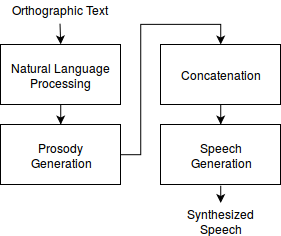
\includegraphics[width=0.6\columnwidth]{tts-structure-0.png}
	\caption{General structure of a \ac{TTS}-system \cite{X}}
\end{figure}

Brief overview of conventional approaches how to implement speech synthesis, with highlighting advantages and drawbacks.

\begin{itemize}[leftmargin=10pt]
	\item concatenative \& unit-selection
	\item formant-based
	\item diphone-based
	\item \ac{SPSS}
	\item etc. ??
\end{itemize}

\vspace{1em}

\begin{itemize}[leftmargin=10pt]
	\item Why speech synthesis is useful/important?\\What are use cases in daily life?
	\item Why there is need to further improve this technology?
\end{itemize}

\subsection{HMM based Speech Synthesis: \ac{SPSS}}
\label{subsec:hmmspeech}

Description of one approach (\ac{SPSS}) more in detail \cite{zen:statistical}.

\clearpage

\section{\ac{SPSS} with Deep Learning Models}
\label{sec:deepspeech}

Description of the improvements of the approach in previous subsection by using deep learning models.

\subsection{General ways for improvement}
\label{subsec:deepeffect}

The effect of neural networks in statistical parametric speech synthesis \cite{hashimoto:effect}

\subsection{One specific approach for improvement}
\label{subsec:deepspss}

Statistical parametric speech synthesis using deep neural networks \cite{zen:deepstatistical}

\section{Speech Synthesis on Embedded Devices}
\label{sec:embeddedspeech}

\subsection{Motivation}
\label{subsec:motembedded}

Why is it important to implement speech synthesis on embedded platform?\\
What needs to be thought about when dealing with embedded or mobile devices?

\subsection{\ac{HMM}-based Approach}
\label{subsec:hmmembedded}

An example of how speech synthesis can be implemented on embedded platform without deep learning (core paper~3).

\subsection{Deep Learning-based Approach}
\label{subsec:deepembedded}

An example of how speech synthesis can be implemented on embedded platform WITH deep learning (core paper 4).

\clearpage
